\documentclass{article}
\usepackage{amsmath}
\usepackage[utf8]{inputenc}
\usepackage[T1]{fontenc}
\usepackage{graphicx}
\graphicspath{ {/home/poiso/uni/primo-anno/Logica-Reti-Logiche-1/} }
\begin{document}
    \section{Logica}
    \begin{flushleft}
       Problema: su un isola ci sono 2 tipi di persone quelle che dicono sempre il vero e quelle che dicono sempre il falso.
       Prendiamo 2 persone da questa isola che chiamiamo A e B, e A dice: "Entrambi di noi siamo falsi". Da questa frase riusciamo a determinare
       che tipo di persone sono A e B? La risposta e' si.
    \end{flushleft}
    \begin{flushleft}
     Prendiamo tutte le combinazioni possibili che si possono formare:T,T; T,F; F,T; F,F\\
     e analizzando caso per caso arriviamo alla conclusione che e' F,T (tenere in conto che il primo valore e riferito ad A e il secondo a B%?
    \end{flushleft}
    \subsection{Logica Proposizionale: Connettivi logici}
    \begin{flushleft}
     La logica proposizionale e' formata da formule i guess, e ognuna di queste formule e formata da variabili e connettivi
     \begin{itemize}
        \item Variabili: p,q,r,...
        \item Connettivi: \begin{itemize}
            \item not $\rightarrow$ ~p oppure $\neg$p%inserire simbolo connettivo
            \item or(inclusivo) $\rightarrow$ p $\lor$ q%inserire simbolo connettivo
            \item implicazione $\rightarrow$ p $\to$ q %inserire simbolo connettivo
            \item equivalenza $\rightarrow$ p $\equiv$ q %inserire simbolo connettivo
            \item xor (or esclusivo)$\rightarrow$ p $\oplus$ q %inserire simbolo connettivo
            \item joint denial: negazione dell' or$\rightarrow$ p $\downarrow$ q %inserire simbolo connettivo
            \item alternative denial: negazione dell' and$\rightarrow$ p $\uparrow$ q %inserire simbolo connettivo
        \end{itemize}
     \end{itemize}
     \subsubsection{Definizioni}
     \begin{itemize}
       \item Definizione di formula:
           \begin{enumerate}
            \item Le variabili sono formule ben definite
            \item se x e' una formula ben definita allora anche ~x e' una formula ben definita
            \item se x e y sono formule ben definite allora anche (x (pallino) f) e' una formula ben definita
           \end{enumerate}
       \item Definzione: Data una formula ben definita x, diciamo che x e':
           \begin{itemize}
            \item Tautologia: se e' sempre vera
            \item Contraddizione: se e' sempre falsa
            \item Condingenza: se puo' essere sia vera che falsa
           \end{itemize}
        \item Definizione: data una formula x, un assegnazione di verita' delle variabili delle formule e' un iterpretazione
        \item Date 2 formule, x e y dicono che:
            \begin{itemize}
               \item x implica logicamente y se x $\to$ y e' tautologia
               \item x e' equivalente a y se x (equivalente) y e' tautologia
            \end{itemize}
       \end{itemize}
    \end{flushleft}
    \section{Metodo dei Tableux}
    \begin{flushleft}
        Il metodo dei tableux e' un metodo che ti permette di verificare se una espressione logicamente
        e' una tautologia,contraddizione o codingenza.Per verificare se e' una condingenza bisogna cominciare
        a lavorare dalla negazione e applicando le seguenti regole:\\
        \begin{tabular} {|p{3cm}||p{3cm}||p{3cm}|}
           \hline
            \multicolumn{3}{|c|}{Formule $\alpha$}\\
           \hline
            $\alpha$& $\alpha_1$& $\alpha_2$ \\
            \hline
            $ X \land Y$& $ X$ & $ Y$ \\
            $\neg(X \lor Y)$& $\neg X$& $\neg Y$ \\
            $\neg(X \to Y)$& $ X$& $\neg Y$ \\
            \hline
        \end{tabular}
        \begin{tabular}{|p{3cm}||p{3cm}||p{3cm}|}
           \hline
            \multicolumn{3}{|c|}{Formule $\beta$}\\
           \hline
            $\beta$& $\beta_1$& $\beta_2$ \\
            \hline
            $ X \lor Y$& $ X$ & $ Y$ \\
            $\neg(X \land Y)$& $\neg X$& $\neg Y$ \\
            $X \to Y$& $ \neg X$& $Y$ \\
            \hline
        \end{tabular}
    \end{flushleft}
    \subsection{Definizioni}
    \begin{itemize}
        \item Diciamo che f e' dimostrabile col metodo di tableux, se partendo da $\neg f$ e distendendo tutte
            le formule otteniamo un tableux chiuso
        \item Un tabluex chiuso se tutti i suoi rami sono chiusi.
        \item Un ramo di un tableux e' chiuso se sul ramo ce sia una formula che la sua negata
    \end{itemize}
    \textbf{Teorema della correttezza}
    \begin{flushleft}
        se F e' dimostrabile col metodo dei tableux allora e' una tautologia
    \end{flushleft}
    \textbf{Teorema della completezza}
    \begin{flushleft}
        Se F e' una tautologi allora e' dimostrabile col metodo dei tableux
    \end{flushleft}
    \begin{itemize}
        \item Diciamo che f e' soddisfacibile se e solo se e' o una tautologia o una contingenza
        \item Un insime S di formule e' soddisfacibile se esiste un interpretazione che soddisfa tutte le formule di S. E.g:
            \begin{equation}
                S=\{p\to q,p \to \neg q, q\to p\}
            \end{equation}
            Questo e' un insieme soddisfacibile
        \item Osservazione: Se f e' un insieme soddisfacibile F e S e' una $\alpha$-formula la cui componenenti sono:
            \begin{equation}
                S_1=S\cup \{F_1,F_2\}
            \end{equation}
        \item Osservazione: Se f e' un insieme soddisfacibile F e S e' una $\beta$-formula con componenti $F_1$ e $F_2$,
            almeno uno tra $S_1$ o $S_2$ e' soddisfacibile:
            \begin{equation}
                S_1=S\cup \{F_1\} \lor  S_2=S\cup \{F_2\}
            \end{equation}
        \item Un ramo di un tableux e' soddisfacibile se l'insieme $S_0$ delle formule sul ramo $\theta$ soddisfacibile.
        \item Un tableux $\tau$ e' soddisfacibile se ha almeno un ramo soddisfacibile
        \item    \textbf{Dimostrazione}: (del teorema di correttezza)\\
            Sia f dimostrabile col metodo di tableux e supponiamo per assurdo che F non e' una tautologia. \\
            Allora c'e' un interpretazione che rende F falsa.
            Allora c'e' un interpretazione che rende F vera se $\neg$F e' soddisfacibile.\\
            Sviluppando il tabluex di $\neg$F ottengo sempre un ramo soddisfacibile. Non e' possibile perche' se F e' dimostrabile
            nel metodo di tableux, tutti i rami sono chiusi.
    \end{itemize}
        \section{Insieme Hintikka}
        \begin{flushleft}
            Un insieme S di formule si chiama insieme di Hintikka se valgono le tre proprieta' seguenti:
            \begin{itemize}
                \item $H_0$: Se non contiene sia una variabile p che la sua negata $\neg$p
                \item $H_1$: Se contiene un $\alpha$-formula allora contiene anche entrambe le sue componenti $\alpha_1,\alpha_2$
                \item $H_2$: Se contiene una $\beta$-formula allora contiene almeno una dell sue componenti $\beta_1,\beta_2$
            \end{itemize}
            \textbf{Osservazione}: Se $\tau$ e' un tabluex "completo" e $\theta$ e' un ramo aperto di $\tau$ allora
            l'insieme $S_\theta$ di tutte le formule sul ramo $\theta$ e' un insieme di Hintikka.
        \end{flushleft}
        \subsection{Lemma di Hintikka}
        \begin{flushleft}
            Se S e' un insieme di Hintikka allora S e' soddisfacibile.
        \end{flushleft}
        \section{Sistemi Assiomatici}
        \begin{flushleft}
         I sistemi assiomatici sono un insieme di leggi o formule che servono per dimostrare una formula. Il sistema assimatico che
          utilizzeremo sara' chiamato $S_0$ e conterra queste formule e regole:
          \begin{equation}
            A_1: \quad x\to (y\to x) \quad A_2: \quad (x\to (y \to z)) \to ((x\to y)\to (x \to z))
            % sarebbe da andare a capo
          \end{equation}
          \textbf{Modus Ponens:}
          \begin{equation}
            \frac{x,x \to y}{y} 
          \end{equation}
          La definizione sopra vuol dire che se noi abbiamo $x$ e $x\to y$ allora abbiamo anche y \\
          \textbf{Osservazione:} Se x e' tautologia e $x \to y$ e' tautologia allora anche y e' tautologia. \\ 
          \textbf{Dimostrazione:} Supponiamo per assurdo che y non e' una tautologia. Allora e' un interpretazione che rend y falsa.
          Siccome x e' tautologia tutte le interpretazioni rendono x vera\\ 
          \textbf{Definzione:} in un Sistema assiomatico S, una dimostrazione di una formula F e' una sequenza di formule $F_1,F_2,...,F_n$ dove $F_n$
          e' f e ogni formula $f_i$ e':
          \begin{itemize}
            \item o un'istanza di un assioma
            \item oppure e' ottenuto da formule precedenti usando le regole di interferenza
          \end{itemize}
          \textbf{Lemma}: Sia F formula qualunque. La formula $F\to F$ e' un teorema nel sistema $S_0$ \\ 
          \textbf{Definizione:} Dato un sistema assiomatico $S_0$ una formula F e un insieme di formule $\Gamma$ una derivazione di F da $\Gamma$
          e' una sequenza di formule $F_1,F_2,...F_n$ tali che $F_n=F$ e ognuna delle F:
          \begin{itemize}
            \item o e' un istanza di un assioma
            \item o si ottiene dalle formule precedenti della sequenza tramite una regola di inteferenza
            \item oppure e' una formula dell insieme $\Gamma$
          \end{itemize}
          \textbf{Osservazione:} Siano F e g 2 formule. Se in $S_0 \{F \} simbolo G$ allora $SimboloF\to g$
        \end{flushleft}
        \subsection{Teorema di Deduzione}
        \begin{flushleft}
          Siano F e G formule e sia $\Gamma$ un insieme di formule, allora se
          \begin{equation}
            \Gamma \cup \{f \}simbolo_{S_0} G \Rightarrow \Gamma simbolo_{S_0} F\to G
          \end{equation}
          Un altro sistema assiomatico che potremmo usare e' lo stesso di prima ma con l aggiunta di $A_3$ che in questo caso e':
          \begin{equation}
            (\neg x \to \neg y)\to((\neg x \to y) \to x) 
          \end{equation}
          L' aggiunta di questa formula fa si che si crea un altro sistema assiomatico che si chiamera' $S_1$
        \end{flushleft}
        \section{Logica del primo ordine}
        \begin{flushleft}
          Esempi:
          \begin{itemize}
            \item Tutti gli uomini sono mortali, Io sono un uomo, Quindi io sono mortale
            \item Tutte le mosche volano, Io sono una mosca, Quindi io volo
          \end{itemize}
          Tutti dicono:
          \begin{itemize}
            \item Siamo tutti dello stesso tipo (Sono tutti true)
            \item C'e' qualcuno di tipo true e qualcuno di tipo false (tutti false)
            \item Tutti quelli di tipo true fumano (tutti true e tutti fumano)
            \item Tutti quelli piu alti di 2 metri, hanno gli occhi verdi (Tutti true anche su insieme vuoto)
            \item Alcuni sono di tipo false e fumatori (tutti false e non fumatori)
          \end{itemize}
          Tutti dello stesso tipo:
          \begin{itemize}
            \item Se qualcuno fuma, allora io fumo (tutti true, nessuno/tutti fumano)
            \item Alcuni sono di tipo false e fumano (tutti true e non fumano)
          \end{itemize}
          P(x) = "x studia"  e Q(x)=" x passa l'esame "
          \begin{itemize}
            \item C'e' qualcuno che studia $\to \quad \exists xP(x)$
            \item Tutti passano l esame $\to \quad \forall xQ(x)$
            \item tutti quelli che studiano passano l'esame \\
                Ipotesi
              \begin{itemize}
              \item $P(x) \to Q(x)$ = se x studia allora passa l'esame (x)
              \item $\forall xP(x) \to Q(x)$ = se tutti studiano allora x passa l'esame (x)
              \item $\forall xP(x) \to \forall Q(x)$ = se tutti studiano allora tutti passano l'esame (x)
              \end{itemize}
              Risposta:
            \item $\forall x [P(x) \to Q(x)]$ 
          \end{itemize}
        \end{flushleft}
        \begin{flushleft}
          Osservazioni:
          \begin{itemize}
            \item $\neg \exists xP(x)\to \forall x \neg P(x)$
            \item $\neg \forall xP(x)\to \exists x \neg P(x)$
          \end{itemize}
        \end{flushleft}
        \subsection{Sintassi e semantica}
        \begin{flushleft}
          I simboli:
          \begin{itemize}
            \item I connettivi
            \item Le variabili individuali
            \item Lettere predicative
            \item I quantificatori 
            \item Le costantin (a,b,c)
            \item Le lettere funzionali (f,g,h)
          \end{itemize}
        \end{flushleft}
        \begin{flushleft}
          \textbf{Def(termini):} Le variabili e le costanti sono termini se $t_1,...,t_n$ sono termini e se $f^n$ e' una funzione di n termini
          allora anche $f^n(t_1,...,t_n) e' termine$
          \textbf{Def(formule ben formate)}:Se $t_1,...,t_n$ sono termini e $p^n$ e' una lettera predicativa con n argomenti allora $p^n(t_1,...,t_n)$ e' fbf
          \begin{itemize}
            \item Se F e' una formula fbf allora anche $\neg$F e' fbf
            \item Se F e G una fbf allora anche $F \circ G$ e' fbf ($\circ$ == qualunque connettivo)
            \item Se F e' una fbf e x e' una variabile anche $\exists xf,\forall xf$ sono fbf
          \end{itemize}
        \end{flushleft}
        \begin{flushleft}
          \textbf{Def(interpretazione):} Data F fbf, un'interpretazione di F e' costituita da:
          \begin{enumerate}
            \item Un dominio
            \item Una relazione o una proprieta' per ognuna delle lettere predicative
            \item Una funzione per ogni lettera funzionale
            \item Un elemento del dominio per ogni costante
          \end{enumerate}
        \end{flushleft}
        \begin{flushleft}
          \textbf{Def(variabili libere e vincolate):} In una formula F una variabile e' vincolata se sta nel raggio di un quantificatore. Altrimenti e' libera
        \end{flushleft}
        \begin{flushleft}
          \textbf{Def(formula chiusa):} Una formula e' chiusa se non ha variabili chiuse. \\ 
          Osservazione: se F e' una formula chiusa allora in una qualunque interpretazione F e' true o false.
        \end{flushleft}
        \begin{flushleft}
          \textbf{Def(formule valie vs tautologie):} Una formula F e' valida se e' vera in ogni interpretazione.  
          \begin{itemize}
            \item Una formula F e' valida se e' vera in ogni interpretazione. 
            \item Una formula f e' tautologia se e' istanza di una tautologia nella logica proposizionale 
          \end{itemize}
        \end{flushleft}
        \subsection{Metodo dei tableux per la logica del primo ordine}
         \subsubsection{Formule universali e esistenziali}
         \begin{itemize}
           \item \textbf{Universali:} Dove a parametro qualunque
             \begin{itemize}
               \item $\forall x P(x) \Rightarrow P(a)$
               \item $\neg \exists x P(x) \Rightarrow \neg P(a)$
             \end{itemize}
           \item \textbf{Esistenziali:} Dove a e' un parametro mai usato prima
             \begin{itemize}
               \item $\exists x P(x) \Rightarrow P(a)$
               \item $\neg \forall x P(x) \Rightarrow \neg P(a)$
             \end{itemize}
         \end{itemize}
         \begin{flushleft}
          \textbf{Osservazione:} Le formule universali si possono sviluppare piu' volte anche con diversi parametri
         \end{flushleft}
         \subsection{Correttezza e Completezza del metodo dei tableux per la logica del primo ordine}
         \begin{flushleft}
           Def: Una formula F e' dimostrabile col metodo dei tableux, se partendo da $\neg$F possiamo ottenere un tableux chiuso
         \end{flushleft}
         \subsubsection{Teorema Correttezza}
         \begin{flushleft}
          Se F e' dimostrabile col metodo dei tableux allora F e' valida:
          \begin{itemize}
            \item Se F non e' valida allora $\neg$F e' soddisfacibile
            \item Se $\neg$F e' soddisfacibile e sviluppo il tableux ci rimmarra' sempre un ramo aperto
            \item Quindi se partendo da $\neg$F ottengo un tableux chiuso allora F e' valida
          \end{itemize}
         \end{flushleft}
         \begin{flushleft}
           \textbf{Lemma}: Sia S un insieme di formule soddisfacibile e sia F $\in$ S una formula
           \begin{enumerate}
             \item Se F e' $\alpha$-formula allora anche $S \cup \{ \alpha_1,\alpha_2\}$ e' soddisfacibile
             \item Se F e' $\beta$-formula allora almeno uno degli insiemi $S \cup \{ \beta_1\}$ o $S\cup \{\beta_2 \}$ e' soddisfacibile
             \item Se F e' $\gamma$-formula allora anche $S \cup \{ \gamma(a)\}$ e' soddisfacibile, qualunque sia il parametro a
             \item Se F e' $\delta$-formula allora anche $S \cup \{ \delta(a)\}$ e' soddisfacibile, se a e' un parametro mai usato prima
           \end{enumerate}
         \end{flushleft}
         \subsubsection{Teorema Completezza}
         \begin{flushleft}
          Se F e' valida allora e dimostrabile col metodo dei tabluex
         \end{flushleft}
         \subsection{Metodo sistematico dello sviluppo del tableux}
         \begin{itemize}
           \item Stabilisci un'ordine per i parametri ($a_1,a_2,a_3$)
           \item Sviluppo le formule nell'ordine in cui compaiono
           \item Usa sempre il primo parametro nell'ordine stabilito
           \item Quando ci sono formule universali, la si puo' sviluppare piu' volte nei rami aperti
         \end{itemize}
         \begin{flushleft}
           Def: Un insieme S di formule e' un insieme di Hintikka se valgono le seguenti proprieta':
           \begin{itemize}
             \item $H_0$: Se non contiene ne $\alpha$ o $\beta$ formule
             \item $H_1$: Se S contiene $\alpha$-formule allora contiene $\alpha_1$ e $\alpha_2$
             \item $H_2$: Se S contiene $\beta$-formule allora contiene o $\beta_1$ o $\beta_2$
             \item $H_3$: Se S contiene $\gamma$-formule allora contiene anche $\gamma$(a) per tutti i parametri a
             \item $H_4$: Se S contiene $\delta$-formule allora contiene anche $\delta$(a) per almeno uno dei parametri a
           \end{itemize}
         \end{flushleft}
         \section{Codifica di complemento a due}
         \begin{flushleft}
          La codifica a complemento a due si fa come una codifica binaria con l unica differenza che l ultimo numero di quando converti il numero
           in binario deve cambiare segno. E.g:
         \end{flushleft}
         \begin{equation}
          -x_32^3+x_22^2+x_12^1+x_02^0
         \end{equation}
         \begin{flushleft}
          Dove le x sono i bit del numero in questo caso un numero in binario di 4 bit. Un esempio puo essere scrivere 5 in complemento a due
         \end{flushleft}
         \begin{equation}
           \begin{split}
             & -x_32^3+x_22^2+  x_12^1+x_02^0=-5 \\ 
              & \iff \\  
              & x_22^2+x_12^1+x_0  2^0=x_32^3-5 \\ 
              & \iff \\
              & x_22^2+x_12^1+x_0  2^0=3 \\ 
           \end{split}
         \end{equation}
         \begin{flushleft}
           Quindi la codifica di -5 sara' (1011)
         \end{flushleft}
          \section{Reti logiche}
          \begin{flushleft}
            Nella logica dei circuiti non scriveremo i simboli come li scrivevamo nella logica proposizionale  e nella logica di primo ordine
          \end{flushleft}
          \begin{itemize}
            \item $ p \land q \to$ pq
            \item $ p \lor q \to$ p+q
            \item $ \neg p \to$ \= p
          \end{itemize}
          \begin{flushleft}
            Ora useremo le porte logiche per scrivere le esporessioni e creare dei circuiti. E in questi circuiti, le porte logiche
            possono avere piu input.
          \end{flushleft}
          \begin{itemize}
            \item Nel caso dell AND l'output sara' 1 se e soltanto se tutti gli input hanno valore 1
            \item Nel caso dell OR l'output sara' 1 se almeno 1 degli input ha valore 1
          \end{itemize}
          \subsection{Forme normali e circuiti}
          \begin{flushleft}
            Una formula si dice formula normale disgiunta (DNF) se e' una disgiunzione di clausole congiuntive
            $C_1 \lor C_2 \lor ... \lor C_n$ dove c sono formule
          \end{flushleft}
          \begin{flushleft}
            Nel linguaggio dei circuiti possiamo chiamare questo tipo di formula somma di prodotti
          \end{flushleft}
          \begin{flushleft}
            Una formula si dice formula normale congiuntiva (CNF) se e' una conginzione di clausole disgiuntive
            $D_1 \land D_2 \land ... \land D_n$ e nel linguaggio dei circuiti si puo' chiamare prodotti di somme
          \end{flushleft}
          \subsection{Circuiti e Operazioni aritmentiche: somma}
          \begin{flushleft}
            
          \end{flushleft}
          \section{Semplificazioni di formule}
          \subsection{Algebra booleana}
          \begin{itemize}
            \item \textbf{Dualita'}: Qualunque uguaglianza vera resta vera se scambiamo gli zeri con gli uni e l'and con l'or
            \item \textbf{Commutativita'}: xy=yx
            \item \textbf{Distributivita'}: (x*y)z=x(y*z)
            \item \textbf{Assorbimento}: x(x+y)=x
            \item \textbf{Combinazione}: xy+x\=y=x
            \item \textbf{Consenso}: xy+\=xz+yz=xy+\=xz
          \end{itemize}
          \subsection{Mappa di Karnaugh}
          \begin{flushleft}
            Un altro metodo per semplificare le formule e' usare il metodo dei
          \end{flushleft}
          \subsection{Blocchi funzionali}
          \begin{flushleft}
            Blocco funzionale e' una porzione di circuito che esegue una specifica funzione
          \end{flushleft}
          \subsubsection{Encoder}
          \begin{flushleft}
            L'Encoder prende $2^n$ input e $n$ output (Inserire immagine encoder)
          \end{flushleft}
          \begin{flushleft}
            La sequenza $(y_2,y_1,y_0)$ dove $y_2$ rappresenta il primo but della sequenza.
            Quindi se mettiamo un "or" all'output $y_2$ dobbiamo collegarci tutti gli input che hanno la combinazione di bit
            che inizia per 1 come per esempio in questo caso 
          \end{flushleft}
          \begin{equation*}
            y_2=x_7+x_6+x_5+x_4
          \end{equation*}
          \subsubsection{Decoder}
          \begin{flushleft}
            Il Decoder e' un altro tipo di circuito che dati $n$ input ha $2^n$ output e ha il seguente funzionamento
          \end{flushleft}
          (immagine del decoder)
          \begin{itemize}
            \item Restituisce 1 se $(x_0,x_1)=i-1$ dove i e' l indice della y $(y_i)$
            \item Restituisce 0 altrimenti
          \end{itemize}
          \subsubsection{Multiplexer}
          \begin{flushleft}
            Questo circuito prende in input $2^n$ variabili e ritorna il valore in output che corrisponde una sequenza di lungezza $n$ $(s_0,s_1)$
            che si chiamano variabili di selezione
          \end{flushleft}
          (immagine multiplexer)
          \begin{flushleft}
            E.g: se $(s_0,s_1)=(0,0)$ il circuito ritornera il valore/variabile $x_0$
          \end{flushleft}
          \subsection{Circuiti sequenziali}
          \begin{flushleft}
            Oss: il D-latch:
          \end{flushleft}
          \begin{itemize}
            \item quando clk=0 l'output resta uguale a quello di prima
            \item quando clk=1 il valore dell'output e' il valore di D
          \end{itemize}
          Oss: Flip Flop:
          \begin{flushleft}
            Fa passare in output il valore dell'input sul fronte di salita$(*)$ del clock
          \end{flushleft}
          \begin{flushleft}
            $(*)$=nel momento in cui clk passa da 0 a 1
          \end{flushleft}
          \begin{flushleft}
            Def: Un registro e' un banco di flip flop collegati allo stesso clock \\ 
            L'architettura a 64 bit dei computer = 64 flip flop \\ 
            Quando si dice che la velocita' del processore e' di 3Ghz vuol dire che il clock cambia valore 3 miliardi di volte al secondo \\ 
            Se all interno di un circuito c'e' un registro allora non ci possono essere paradossi logici
          \end{flushleft}
          \begin{flushleft}
            IL resto leggere gli appunti del prof (https://www.mat.uniroma2.it/~pasquale/dida/aa2324/lrl/ep14.pdf)
          \end{flushleft}
          \section{Codifica numeri in virgola mobile}
          \subsection{ Standard IEEE 754}
          \subsubsection*{IEEE 754 a precisione singola (32 bit)}
          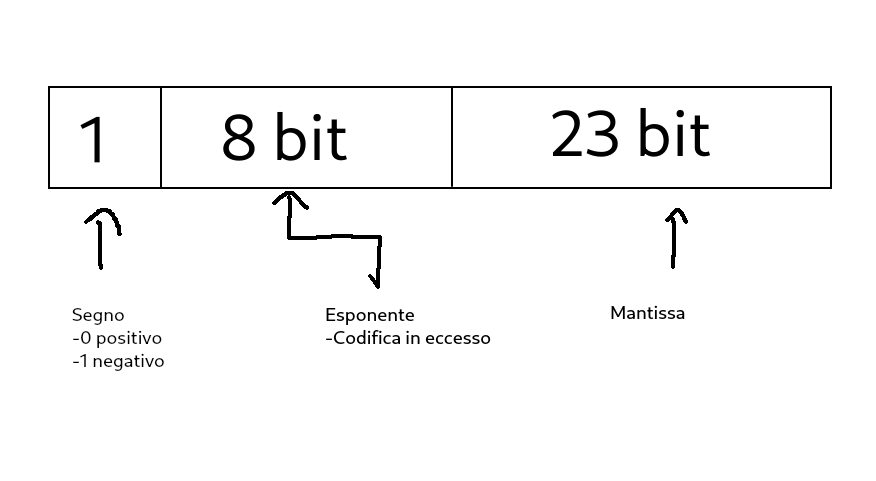
\includegraphics[bb=0 0 250 200]{pic/ieee32bit.png}
          \subsubsection*{IEEE 754 a precisione doppia (64 bit)}
          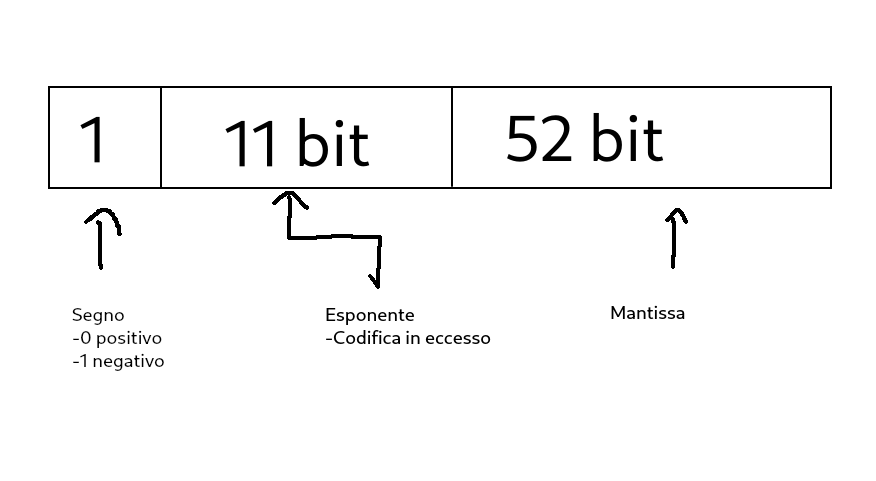
\includegraphics[bb=0 0 250 200]{pic/ieee64bit.png}
          \subsection{Come funziona la codifica IEEE 754}
          \begin{flushleft}
           Come possiamo vedere dalle immagini sopra la codifica e divisa in 3 settori
          \end{flushleft}
          \begin{itemize}
            \item Il segno 
            \item l esponente
            \item la mantissa
          \end{itemize}
          \begin{flushleft}
            \textbf{Il segno} ha un solo bit a disposizione dove se il bit e' impostato a 1 
            vuol dire che il numero e' negativo altrimenti e' positivo
          \end{flushleft}
          \begin{flushleft}
            \textbf{L'esponente} ha a disposzione 8 bit nella versione a 32 bit del IEEE e 11 bit
            invece nella versione a 64 bit. In questi bit viene salvato il numero che elevato alla
            2 ci riportera al numero originale (perche durante la conversione noi prendiamo il numero
            in binario e lo portiamo ad una versione del tipo e.g $1,011101 * 2^6$) dove poi l'esponente
            sara codificato in codifica ad eccesso, cioe' il numero trovato prima di convertirlo in binario
            dovra' essere addizionato a 127 e poi essere convertito. Nella decodifica invece una volta tradotto
            il numero da binario a decimale si dovra sottrarre 127.
          \end{flushleft}
          \begin{flushleft}
            \textbf{La mantissa} e' composta da 23 bit nella versione a precisione singola e 52 bit
            nella versione a precisione doppia. In questa parte della codifica viene salvata la parte
            prima della virgola del numero quando si vorra trovare l esponente e.g $1,011101 * 2^6$
            cioe' l'esempio di prima, nella parte riservaata all'esponente verra' salvato 133 in binario
            e nella parte della mantissa verra salvato "011101"
          \end{flushleft}
          \begin{flushleft}
            Una volta che avremmo la nostra sequenza binaria dovremmo convertirla in esadecimale 
            prendendo 4 bit alla volta e convertendoli in esadecimale 
          \end{flushleft}
          \begin{flushleft}
            Per decodificare un numero scritto con lo standard IEEE si puo' agire intuitivamente
            facendo analogamente l'opposto della codifica
          \end{flushleft}
           \subsection{Numeri particolari} 
           \begin{flushleft}
            Queste sono particolari sequenze di bit che di conseguenza hanno valori particolari
           \end{flushleft}
           \begin{itemize}
             \item 0
               \begin{itemize}
                 \item Qualsiasi bit per il segno
                 \item Tutti i bit a 0 per l'esponente
                 \item Tutti i bit a 0 per la mantissa
               \end{itemize}
             \item $+\infty$
               \begin{itemize}
                 \item Il bit del segno impostato a 0
                 \item Tutti i bit a 1 per l'esponente
                 \item Tutti i bit a 0 per la mantissa
               \end{itemize}
             \item $-\infty$
               \begin{itemize}
                 \item Il bit del segno impostato a 1
                 \item Tutti i bit a 1 per l'esponente
                 \item Tutti i bit a 0 per la mantissa
               \end{itemize}
             \item NaN (Not a Number)
               \begin{itemize}
                 \item Qualsiasi bit per il segno
                 \item Tutti i bit a 1 per l'esponente
                 \item Una sequenza di bit diversa da 0
               \end{itemize}
           \end{itemize}
          \section{Codificare caratteri}
          \begin{flushleft}
            Negli anni 60 fu inventata la codifica ad ASCII che permetteva di codificare $2^7$ caratteri ( per un totale di 128 caratteri) 
          \end{flushleft}
          \begin{flushleft}
            Questo codifica non fu standardizzata perche' molti paesi hanno caratteri differenti da utilizzare
            quindi ogni continente/paese aveva un modo per codificare i caratteri diverso dagli altri
          \end{flushleft}
          \begin{flushleft}
            Negli ultimi anni e stato pero standarzittato un nuovo "modo" che si chiama unicode che codifica
            da 0x000000 a 0xFFFFFF
          \end{flushleft}
          \begin{flushleft}
            Le codifiche che implementano questo nuovo metodo sono le UTF (utf-8,16,32) quella piu' utilizzata al momento e' utf-8
            ed e' una codifica a lunghezza variabile 
          \end{flushleft}
          \begin{flushleft}
           La codifica sfrutta 1 byte che inizia tanti 1 quanto e' il numero di byte utilizzato da un carattere questa sequenza poi termina con 0 
           poi per il resto del byte verra' occupato dalla codifica del carattere gli altri byte sucessivi inizieranno con la sequenza 10
          \end{flushleft}
          E.g
          \begin{flushleft}
            1 byte \quad     1 0 - - - - - - \quad \\
            2 byte  \quad    1 1 0 - - - - -      \quad 1 0 - - - - - - \\
            3 byte  \quad    1 1 1 0 - - - -      \quad 1 0 - - - - - - \quad       1 0 - - - - - - \\
            4 byte  \quad    1 1 1 1 0 - - -      \quad 1 0 - - - - - -      \quad 1 0 - - - - - -     \quad 1 0 - - - - - -\\
          \end{flushleft}
        \end{document}
